\documentclass[
	classe=$2^{de}$
]{évaluation}

\usepackage{tcolorbox}
\usepackage{tikz-repère}

% First one is correct
\newcommand{\correctionStrike}[2]{%
\ifdefined\makeCorrection%
\sout{#1}/#2
\else%
#1/#2
\fi%
}

\newcommand{\DotsForCorrection}{....................}

\date{5 mai 2023}

\begin{document}

\title{Évaluation : fonctions (sujet A)}
\maketitle

\begin{tcolorbox}
	Les exercices $1$, $3$ et la question $3$ de l'exercice $4$ sont à faire sur le sujet, le reste est à faire sur une feuille à part.

	La calculatrice est autorisée.

	Le barème est donné à titre indicatif.
\end{tcolorbox}

\begin{exercice}[2]
	On dispose d'une fonction $f$, telle que
	\begin{align*}
		f(-1) & = 2 & f(0) & = 1 & f(1) & = 6 & f(2) & = 2 & f(3) & = -1 & f(4) & = 6
	\end{align*}
	Remplir :
	\begin{multicols}{2}
		\begin{itemize}
			\item[] $-1$ est \correctionOr{un antécédent}{\DotsForCorrection} de $2$
			\item[] $-1$ est \correctionOr{l'image}{\DotsForCorrection} de $3$
			\item[] \correctionOr{$1$ et $4$}{\DotsForCorrection} sont les antécédents de $6$
			\item[] \correctionOr{$6$}{\DotsForCorrection} est l'image de $1$
		\end{itemize}
	\end{multicols}
\end{exercice}

\begin{exercice}[3]
	Calculer :
	\begin{enumerate}
		\item $f(4)$ pour $f(x) = x - 3$
		\item $f(-1)$ pour $f(x) = \dfrac{5x + 1}{x - 3}$
		\item $f(7)$ pour $f(x) = x^3 - x^2$
	\end{enumerate}
\end{exercice}

\begin{exercice}[4]
	Donner l'expression de chacune de ces fonctions affines, et calculer alors l'image de $100$ :
	\pgfmathsetmacro\scale{0.7}
	\begin{multicols}{2}
		\begin{center}
			\begin{tikzpicture}[scale=\scale]
				\tikzRepere{-3.5}{3.5}{-2.5}{2.5}
				\draw[domain=-4:4,thick,blue] plot({\x},{0.5*\x+1});
			\end{tikzpicture}
			$$ f(x) = \correctionOr{}{\DotsForCorrection} \hspace{2em} f(100) = \correctionOr{}{\DotsForCorrection} $$
		\end{center}

		\begin{center}
			\begin{tikzpicture}[scale=\scale]
				\tikzRepere{-3.5}{3.5}{-2.5}{2.5}
				\draw[domain=-1.5:1.5,thick,blue] plot({\x},{2*\x});
			\end{tikzpicture}
			$$ g(x) = \correctionOr{}{\DotsForCorrection} \hspace{2em} g(100) = \correctionOr{}{\DotsForCorrection} $$
		\end{center}

		\columnbreak

		\begin{center}
			\begin{tikzpicture}[scale=\scale]
				\tikzRepere{-3.5}{3.5}{-2.5}{2.5}
				\draw[domain=-2:1,thick,blue] plot({\x},{-2*\x-1});
			\end{tikzpicture}
			$$ h(x) = \correctionOr{}{\DotsForCorrection} \hspace{2em} h(100) = \correctionOr{}{\DotsForCorrection} $$
		\end{center}

		\begin{center}
			\begin{tikzpicture}[scale=\scale]
				\tikzRepere{-3.5}{3.5}{-2.5}{2.5}
				\draw[domain=-1:4,thick,blue] plot({\x},{\x-2});
			\end{tikzpicture}
			$$ i(x) = \correctionOr{}{\DotsForCorrection} \hspace{2em} i(100) = \correctionOr{}{\DotsForCorrection} $$
		\end{center}

	\end{multicols}
\end{exercice}

\newpage

\begin{exercice}[7]
	\begin{center}
		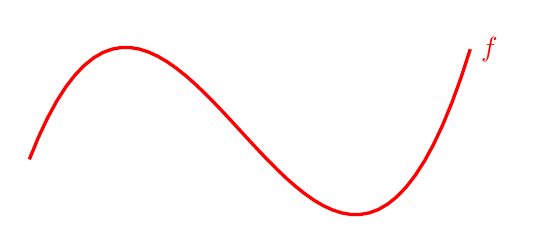
\begin{tikzpicture}[scale=0.7]
			\tikzRepere{-4.5}{4.5}{-2.5}{1.5}
			\draw[domain=-4:0,very thick,red] plot({\x},{1/3*(0.25*\x*\x*\x + 0.125*\x*\x - 3.25*\x - 2)});
			\draw[domain=0:4,very thick,red] plot({\x},{1/3*(0.25*\x*\x*\x + 0.125*\x*\x - 3.25*\x - 2)}) node[right] {$f$};
		\end{tikzpicture}
	\end{center}

	\begin{enumerate}
		\item Quel est le domaine de définition de $f$ ?
		\item Lire :
		      \begin{enumerate}
			      \item L'image de $-4$ par $f$
			      \item Les antécédents de $1$ par $f$
			      \item la valeur de $f(2)$
		      \end{enumerate}
		\item Établir le tableau de variations de $f$.
	\end{enumerate}
\end{exercice}

\begin{exercice}[7]
	On lance une balle dans les airs, et on souhaite étudier sa trajectoire. On lance la balle en l'abscisse $0$ vers le haut, à $50$cm du sol.

	On admet que la trajectoire de la balle est une parabole : sa hauteur en fonction de son abscisse est donnée par la fonction $f(x) = -\dfrac{1}{40}x^2 + 2x + a$, où $a$ est un paramètre à déterminer.

	(Remarque : toutes les unités sont des centimètres dans cet exercice)

	\begin{enumerate}
		\item D'après l'énoncé, quelle est la hauteur de la balle en l'abscisse $0$ ? Que peut-on alors dire de $f(0)$ ?
		\item En utilisant l'expression de $f$, déterminer alors la valeur du paramètre $a$.
		\item Représenter la fonction dans le repère suivant :
		      \begin{center}
			      \begin{tikzpicture}[scale=0.9]
				      \pgfmathsetmacro\scale{10}
				      \tikzRepere{0}{11}{0}{10}[\scale][\scale][abscisse (cm)][hauteur (cm)]

				      \ifdefined\makeCorrection
					      \draw[domain=0:10,very thick,red] plot({\x},{(-0.025*\x*\x*\scale*\scale + 2*\x*\scale + 50)/\scale});
				      \fi
			      \end{tikzpicture}
		      \end{center}
		\item Établir le tableau de variations de $f$.
		\item Lire alors sur le repère :
		      \begin{enumerate}
			      \item Quelle est la hauteur maximale atteinte par la balle ?
			      \item Quelle est l'abscisse à laquelle la balle est retombée sur le sol ?
		      \end{enumerate}
	\end{enumerate}
\end{exercice}

%===========================================
%================ SUJET B ==================
%===========================================

\newpage\setcounter{exercice}{1}

\title{Évaluation : fonctions (sujet B)}
\maketitle

\begin{tcolorbox}
	Les exercices $1$, $3$ et la question $3$ de l'exercice $4$ sont à faire sur le sujet, le reste est à faire sur une feuille à part.

	La calculatrice est autorisée.

	Le barème est donné à titre indicatif.
\end{tcolorbox}

\begin{exercice}[2]
	On dispose d'une fonction $f$, telle que
	\begin{align*}
		f(-2) & = 2 & f(-1) & = 1 & f(0) & = 6 & f(1) & = 2 & f(2) & = -1 & f(3) & = 6
	\end{align*}
	Remplir :
	\begin{multicols}{2}
		\begin{itemize}
			\item[] $-1$ est \correctionOr{un antécédent}{\DotsForCorrection} de $1$
			\item[] $-1$ est \correctionOr{l'image}{\DotsForCorrection} de $2$
			\item[] \correctionOr{$1$ et $4$}{\DotsForCorrection} sont les antécédents de $6$
			\item[] \correctionOr{$6$}{\DotsForCorrection} est l'image de $1$
		\end{itemize}
	\end{multicols}
\end{exercice}

\begin{exercice}[3]
	Calculer :
	\begin{enumerate}
		\item $f(3)$ pour $f(x) = x - 2$
		\item $f(-1)$ pour $f(x) = \dfrac{3x + 1}{x + 2}$
		\item $f(5)$ pour $f(x) = x^3 - x^2$
	\end{enumerate}
\end{exercice}

\begin{exercice}[4]
	Donner l'expression de chacune de ces fonctions affines :
	\pgfmathsetmacro\scale{0.7}
	\begin{multicols}{2}
		\begin{center}
			\begin{tikzpicture}[scale=\scale]
				\tikzRepere{-3.5}{3.5}{-2.5}{2.5}
				\draw[domain=-1.5:1.5,thick,blue] plot({\x},{2*\x});
			\end{tikzpicture}
			$$ f(x) = \correctionOr{}{\DotsForCorrection} \hspace{2em} f(100) = \correctionOr{}{\DotsForCorrection} $$
		\end{center}

		\begin{center}
			\begin{tikzpicture}[scale=\scale]
				\tikzRepere{-3.5}{3.5}{-2.5}{2.5}
				\draw[domain=-4:4,thick,blue] plot({\x},{0.5*\x+1});
			\end{tikzpicture}
			$$ g(x) = \correctionOr{}{\DotsForCorrection} \hspace{2em} g(100) = \correctionOr{}{\DotsForCorrection} $$
		\end{center}

		\columnbreak

		\begin{center}
			\begin{tikzpicture}[scale=\scale]
				\tikzRepere{-3.5}{3.5}{-2.5}{2.5}
				\draw[domain=-1:4,thick,blue] plot({\x},{\x-2});
			\end{tikzpicture}
			$$ h(x) = \correctionOr{}{\DotsForCorrection} \hspace{2em} h(100) = \correctionOr{}{\DotsForCorrection} $$
		\end{center}

		\begin{center}
			\begin{tikzpicture}[scale=\scale]
				\tikzRepere{-3.5}{3.5}{-2.5}{2.5}
				\draw[domain=-2:1,thick,blue] plot({\x},{-2*\x-1});
			\end{tikzpicture}
			$$ i(x) = \correctionOr{}{\DotsForCorrection} \hspace{2em} i(100) = \correctionOr{}{\DotsForCorrection} $$
		\end{center}
	\end{multicols}
\end{exercice}

\newpage

\begin{exercice}[4]
	\begin{center}
		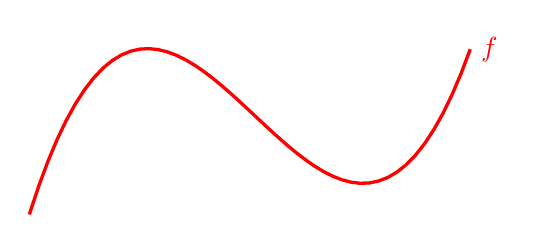
\begin{tikzpicture}[scale=0.7]
			\tikzRepere{-4.5}{4.5}{-2.5}{1.5}
			\draw[domain=-4:0,very thick,red] plot({\x},{1/9*(0.7375*\x*\x*\x - 0.2125*\x*\x - 8.425*\x - 1.1)});
			\draw[domain=0:4,very thick,red] plot({\x},{1/9*(0.7375*\x*\x*\x - 0.2125*\x*\x - 8.425*\x - 1.1)}) node[right] {$f$};
		\end{tikzpicture}
	\end{center}

	\begin{enumerate}
		\item Quel est le domaine de définition de $f$ ?
		\item Lire :
		      \begin{enumerate}
			      \item L'image de $-4$ par $f$
			      \item Les antécédents de $1$ par $f$
			      \item la valeur de $f(1)$
		      \end{enumerate}
		\item Établir le tableau de variations de $f$.
	\end{enumerate}
\end{exercice}

\begin{exercice}[7]
	On lance une balle dans les airs, et on souhaite étudier sa trajectoire. On lance la balle en l'abscisse $0$ vers le haut, à $48$cm du sol.

	On admet que la trajectoire de la balle est une parabole : sa hauteur en fonction de son abscisse est donnée par la fonction $f(x) = -\dfrac{1}{50}x^2 + 2x + a$, où $a$ est un paramètre à déterminer.

	(Remarque : toutes les unités sont des centimètres dans cet exercice)

	\begin{enumerate}
		\item D'après l'énoncé, quelle est la hauteur de la balle en l'abscisse $0$ ? Que peut-on alors dire de $f(0)$ ?
		\item En utilisant l'expression de $f$, déterminer alors la valeur du paramètre $a$.
		\item Représenter la fonction dans le repère suivant :
		      \begin{center}
			      \begin{tikzpicture}[scale=0.9]
				      \pgfmathsetmacro\scale{10}
				      \tikzRepere{0}{13}{0}{12}[\scale][\scale][abscisse (cm)][hauteur (cm)]

				      \ifdefined\makeCorrection
					      \draw[domain=0:12,very thick,red] plot({\x},{(-1/50*\x*\x*\scale*\scale + 2*\x*\scale + 48)/\scale});
				      \fi
			      \end{tikzpicture}
		      \end{center}
		\item Établir le tableau de variations de $f$.
		\item Lire alors sur le repère :
		      \begin{enumerate}
			      \item Quelle est la hauteur maximale atteinte par la balle ?
			      \item Quelle est l'abscisse à laquelle la balle est retombée sur le sol ?
		      \end{enumerate}
	\end{enumerate}
\end{exercice}

\end{document}